%mainfile: GANs.tex

\makeatletter
\patchcmd{\beamer@sectionintoc}
  {\vfill}
{\vskip\itemsep\vspace{0.2em}}
  {}
  {}
\makeatother 

\title[Generative Adversarial Networks]
      {Generative Adversarial Networks (GANs)}
\author{Yu-Guan Hsieh}
\date{January 2018}

\frame{\titlepage}

\begin{frame}
  \frametitle{Plan}
  \begin{columns}
    \column{.06\textwidth}
    \column{.88\textwidth}
    \tableofcontents[]
    \column{.06\textwidth}
  \end{columns}
\end{frame}

\section{Problem Setting}

\begin{frame}
  \frametitle{Problem Setting}
  \begin{columns}
    \column{.06\textwidth}
    \column{.88\textwidth}
    Given a set of real data examples $\{x^{(i)}\}_{i=1}^m\in\mathcal{X}^m$,
    we suppose they come from some real data distribution $\mathbb{P}_r$ and
    we would like to `learn' this probability distribution.
    \column{.06\textwidth}
  \end{columns}
\end{frame}

\section{Maximum Likelihood}

\begin{frame}
  \frametitle{Maximum Likelihood}
  \begin{itemize}
    \item A generative model parameterized by some vector
      $\theta\in\mathbb{R}^d$.
    \item Note $\mathbb{P}_g$ the generator's distribution, supposed to be
      continuous, and $P_g$ its density. Since the model is parameterized
      by $\theta$ here, they'll also be noted $\mathbb{P}_{\theta}$ and
      $P_{\theta}$ for clarity.
    \item We want to find solution of the problem
      \[
        \max_{\theta\in\mathbb{R}^d}\frac{1}{m}\log P_{\theta}(x^{(i)}).
      \]
    \item This amounts to minimize the \textbf{Kullback-Leibler (KL)
      divergence} between $\mathbb{P}_r$ and $\mathbb{P}_{\theta}$:
      \[ 
        KL(\mathbb{P}_r\|\mathbb{P}_{\theta})
        = \int_{\mathcal{X}} P_r(x)\log\frac{P_r(x)}{P_{\theta}(x)} dx,
      \]
      where $P_r$ is the density of $\mathbb{P}_r$ supposing it's continuous.
  \end{itemize}
\end{frame}

\section{Generative Adversarial Network}

\begin{frame}
  \frametitle{Generative Adversarial Network - Setting}
  \begin{itemize}
    \item First appears in 
      ``Ian J. Goodfellow et al. Generative adversarial nets. \textit{Advances
      in Neural Information Processing Systems}, 2014''.
    \item Define a random variable $Z$ with a fixed distribution $\mathbb{P}_z$
      taking values in $\mathcal{Z}$ (ex: a multivariate gaussian) and some
      \textbf{generator} $G: \mathcal{Z} \rightarrow \mathcal{X}$ that
      directly generates samples following a certain distribution
      $\mathbb{P}_g$.
    \item The generator is trained adversarially using a discriminator
      $D: \mathcal{X} \rightarrow [0, 1]$ which indicates the
      \textbf{probability} that
      a certain example $x$ comes from the data rather than $\mathbb{P}_g$.
  \end{itemize}
\end{frame}

\begin{frame}
  \frametitle{Generative Adversarial Network - Objectif}
  \begin{itemize}
    \item Define the function
      \[ 
        V(G, D)
        = \mathbb{E}_{x\sim\mathbb{P}_r}[\log D(x)]
        + \mathbb{E}_{z\sim\mathbb{P}_z}[\log(1-D(G(z)))].
      \]
      The goal is to solve $\min_G\max_D V(G, D)$.
    \item In practice, $D$ and $G$ are two neural networks so alternatively
      we attempt to solve $\max_D V(G, D)$ fixing G and $\min_G V(G, D)$ fixing
      D by computing the gradients.
    \item Instead of minimizing
      $\mathbb{E}_{z\sim\mathbb{P}_z}[\log(1-D(G(z)))]$
      we would rather maximize $\mathbb{E}_{z\sim\mathbb{P}_z}[\log D(G(z))]$.
  \end{itemize}
\end{frame}

\begin{frame}
  \frametitle{Generative Adversarial Network - Illustration}
    \begin{figure}
      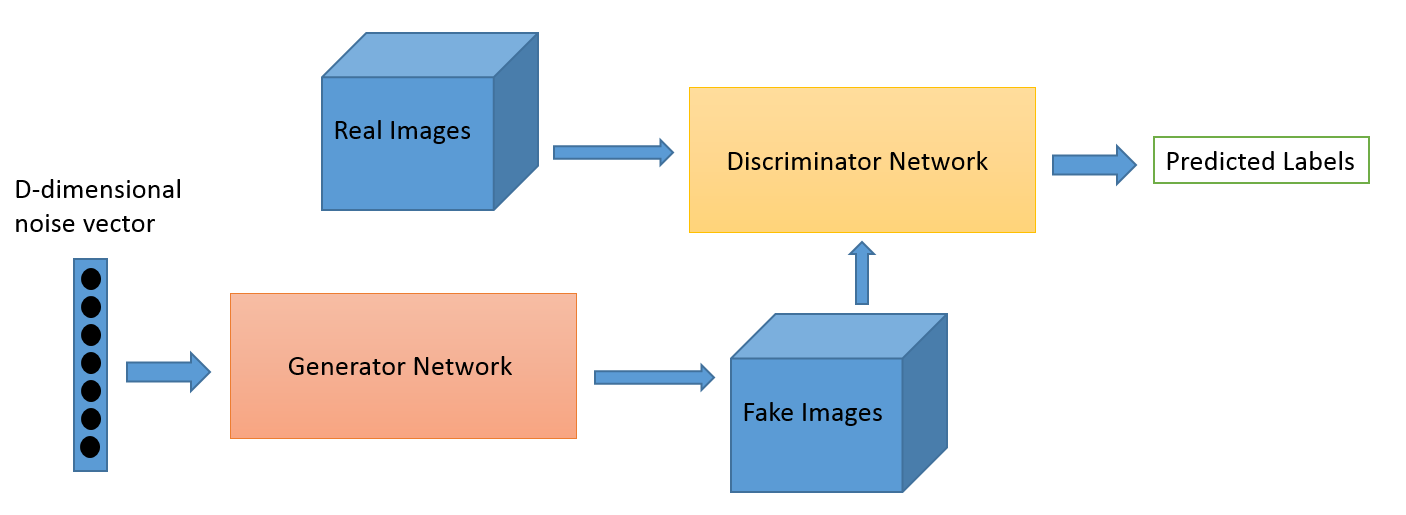
\includegraphics[width=\linewidth]{GAN}
    \end{figure}
\end{frame}

\begin{frame}
  \begin{algorithm}[H]
  \begin{algorithmic}[1]
    \begin{small}
    \FOR{number of training iterations}
      \FOR{$k$ steps}
        \STATE Sample $\{x^{(i)}\}_{i=1}^m \sim \mathbb{P}_r$ a batch
          from real data.
        \STATE Sample $\{z^{(i)}\}_{i=1}^m \sim \mathbb{P}_z$ a batch
          of prior samples.
        \STATE Update the discriminator by ascending its stochastic gradient:
          \[
            \nabla_w\frac{1}{m}
            \sum_{i=1}^m[\log D_w(x^{(i)})
            +\log(1-D_w(G_{\theta}(z^{(i)})))].
          \]
      \ENDFOR
      \STATE Sample $\{z^{(i)}\}_{i=1}^m \sim \mathbb{P}_z$ a batch
        of prior samples.
      \STATE Update the generator by ascending its stochastic gradient:
        \[
          \nabla_{\theta}\frac{1}{m}
          \sum_{i=1}^m \log D_w(G_{\theta}(z^{(i)})).
        \]
    \ENDFOR
    \end{small}
  \end{algorithmic}
    \caption{Training of classic GAN ($D$ and $G$ are respectively
      parameterized by $w$ and $\theta$ and are noted $D_w$ and
      $G_{\theta}$).}
  \end{algorithm}
\end{frame}

\begin{frame}
  \frametitle{Generative Adversarial Network - Theory}
  \begin{itemize}
    \item If $D$ and $G$ are arbitrary functions, when $D$ is trained to its
      optimum for some fixed $G$, we have
      \[ 
        D_G^*(x) = \frac{P_r(x)}{P_r(x) + P_g(x)}.
      \]
    \item Note $C(G) = \max_D V(G, D)$ and
      $\mathbb{P}_m = (\mathbb{P}_r+\mathbb{P}_g)/2$ (mixture
      with densities $(P_r+P_g)/2$), we can show that
      \[
        C(G) = -\log(4) + KL(\mathbb{P}_r \| \mathbb{P}_m) 
        + KL(\mathbb{P}_g \| \mathbb{P}_m).
      \]
    \item We recognize in the previous expression the \textbf{Jensen-Shannon
      (JS) divergence} between the model's distribution and the data
      generating process:
      \[ C(G) = -\log(4) + 2 \cdot JS(\mathbb{P}_r\|\mathbb{P}_g). \]
    \item Minimize the JS divergence between $\mathbb{P}_g$ and $\mathbb{P}_r$.
  \end{itemize}
\end{frame}

\begin{frame}
  \frametitle{Generative Adversarial Network - Defects}
  \begin{itemize}
    \item Need of synchronization between $D$ and $G$ -- we
      \textbf{shouldn't} train the discriminator till convergence. 
    \item Training is very unstable. Choice of architectures rely on
      heuristics that are extremely sensitive to modifications (batch
      normalization, dropout, \dots).
    \item In ``Alec Radford et al. Unsupervised Representation Learning
      with Deep Convolutional Generative Adversarial Networks.
      \textit{ArXiv preprint arXiv:1511.06434}, 2015'', the authors propose
      some architectures of GANs that perform quite well in general.
  \end{itemize}
\end{frame}

\begin{frame}
  \frametitle{Generative Adversarial Network - Results}
  \begin{itemize}
    \item DCGAN (reported in the DCGAN paper).
      \begin{figure}
        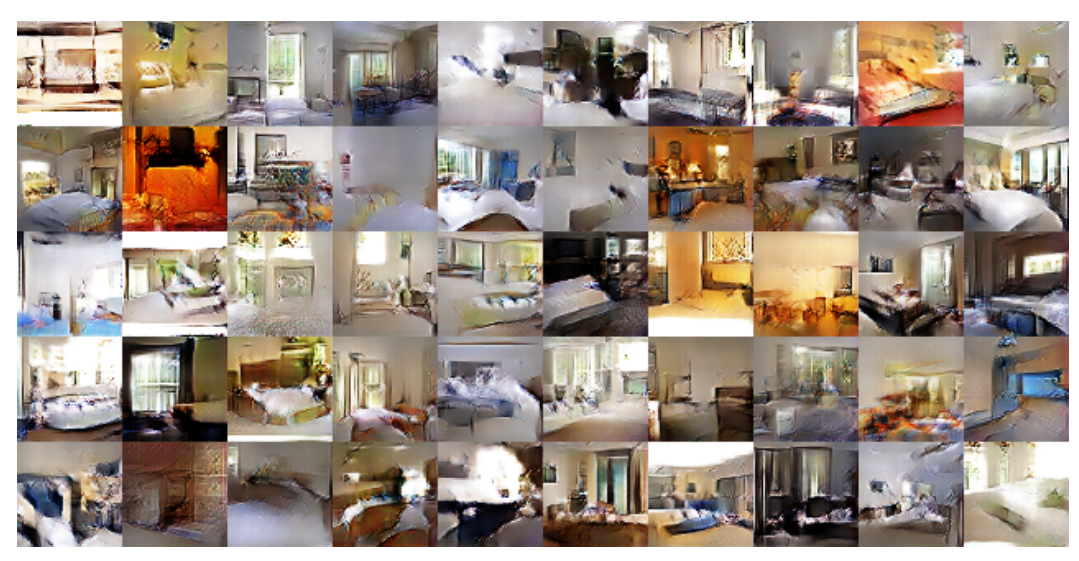
\includegraphics[width=0.9\linewidth]{DCGAN}
      \end{figure}
  \end{itemize}
\end{frame}

\begin{frame}
  \frametitle{Generative Adversarial Network - Results}
  \begin{itemize}
    \item DCGAN without batch normalization in $G$
      (reported in the LSGAN paper).
      \begin{figure}
        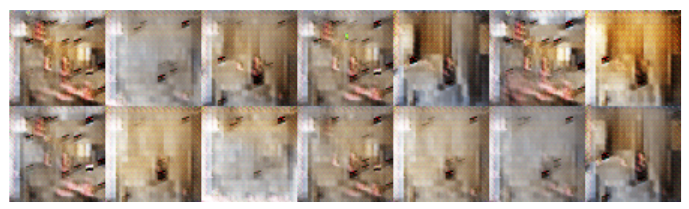
\includegraphics[width=0.75\linewidth]{DCGAN3}
      \end{figure}
    \item Generator without batch normalization and constant number of filters
      at every layer, as opposed to duplicating them every time as for a normal
      DCGAN generator (reported in the WGAN paper).
      \begin{figure}
        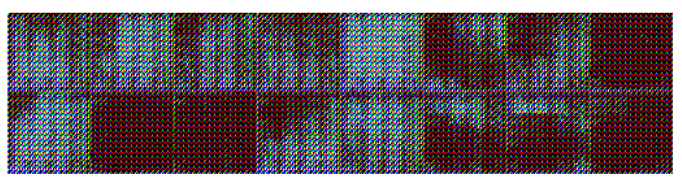
\includegraphics[width=0.8\linewidth]{DCGAN2}
      \end{figure}
  \end{itemize}
\end{frame}

\section{Wassertein GAN}

\begin{frame}
  \frametitle{Wassertein GAN - Theory}
  \begin{itemize}
    \item Consider the Earth-Mover (EM) or Wasserstein distance between
      $\mathbb{P}_r$ and $\mathbb{P}_g$:
      \[
        W(\mathbb{P}_r, \mathbb{P}_g)
        = \inf_{\gamma\in\Pi(\mathbb{P}_r, \mathbb{P}_g)}
        \mathbb{E}_{(x,y)\sim\gamma}[\|x-y\|],
      \]
      where $\Pi(\mathbb{P}_r, \mathbb{P}_g)$ denotes the set of all joint
      distributions $\gamma(x, y)$ whose marginals are respectively
      $\mathbb{P}_r$ and $\mathbb{P}_g$.
    \item When $G$ is a feedforward neural network parameterized by some
      vector $\theta$ (noted $G_{\theta}$ in this case),
      $W(\mathbb{P}_r, \mathbb{P}_{\theta})$ is \textbf{continuous everywhere,
      and differentiable almost everywhere}. This is not the case for neither
      the JS nor any KLs.
  \end{itemize}
\end{frame}

\begin{frame}
  \frametitle{Wassertein GAN - Theory}
  \begin{itemize}
    \item We generally believe that the supports of $\mathbb{P}_r$ and
      $\mathbb{P}_g$ lie in two low dimensional manifolds that have a
      intersection of measure zero. In this case, the KL divergence is
      not defined and the JS divergence equals always $\log2$ and doesn't
      provide any usable gradient information.
    \item The topology induced by Wasserstein distance is weaker than the one
      induced by the JS divergence. That is, for any $\mathbb{P}$
      probability distribution on $\mathcal{X}$ and any
      $(\mathbb{P}_n)_{n\in\mathbb{N}}$ sequence of probability distributions
      over $\mathcal{X}$,
      \[
        JS(\mathbb{P}_n, \mathbb{P})\xrightarrow[n\rightarrow\infty]{}0
        \Longrightarrow
        W(\mathbb{P}_n, \mathbb{P})\xrightarrow[n\rightarrow\infty]{}0.
      \]
    \item The EM distance should be a sensible cost function when learning
      distribution supported by low dimensional manifolds.
  \end{itemize}
\end{frame}

\begin{frame}
  \frametitle{Wassertein GAN - Training}
  \begin{itemize}
    \item By the Kantorovich-Rubinstein duality, for any $K > 0$,
      \[
        W(\mathbb{P}_r, \mathbb{P}_g)
        = \frac{1}{K} \left( \sup_{\|f\|_L \le K}
        \mathbb{E}_{x\sim\mathbb{P}_r}[f(x)]
        - \mathbb{E}_{x\sim\mathbb{P}_g}[f(x)]
        \right)
      \]
      where the supremum is taken over all the $K$-Lipschitz functions
      $f: \mathcal{X} \rightarrow \mathbb{R}$.
    \item In practice, $f$ is another neural network parameterized with
      weights $w$ (thus noted $f_w$ hereinafter) lying in a compact space
      $\mathcal{W}$. The fact that $\mathcal{W}$ is compact
      implies that all possible $f$ will be $K$-Lipschitz for some $K$ that
      only depends on $\mathcal{W}$ and not the individual weights.
    \item In order to have parameters $w$ lie in a compact space, we can for
      example clamp the weights to a fixed box after each gradient update.
  \end{itemize}
\end{frame}

\begin{frame}
  \frametitle{Wassertein GAN - Training}
  \begin{itemize}
    \item We train the `critic' $f_w$ to optimality and carry
      out an update step of $G_{\theta}$ by turns.
    \item By using the formula of last page, we get an estimate of the quantiy
      $K \cdot W(\mathbb{P}_r, \mathbb{P}_g)$. \textbf{This estimate correlates
      well with the quality of the generated samples.}
    \item Such property doesn't exist for the classic GAN.
    \item No more mode collapse.
    \item Work with more architectures.
    \item NB: Use of momentum based optimizer such as Adam on the critic makes
      WGAN training unstable -- use RMSProp instead.
  \end{itemize}
\end{frame}

\begin{frame}
  \frametitle{Wassertein GAN - Results}
  \begin{itemize}
    \item DCGAN architecture.
      \begin{figure}
        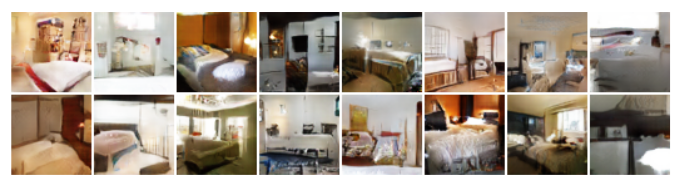
\includegraphics[width=0.8\linewidth]{WGAN1}
      \end{figure}
    \item MLP generator with 4 layers and 512 units with ReLU nonlinearities.
      \begin{figure}
        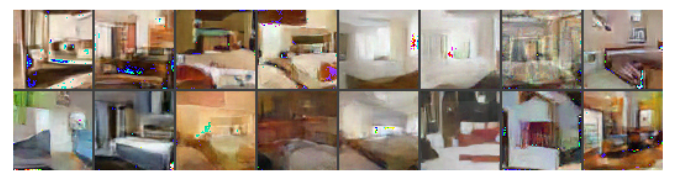
\includegraphics[width=0.8\linewidth]{WGAN2}
      \end{figure}
  \end{itemize}
\end{frame}

\section{Other Variants}

\begin{frame}
  \frametitle{Least Squares GAN}
  \begin{itemize}
    \item Replace the sigmoid cross entropy loss function with the least
      squares loss function. We fix some $a-b$ coding scheme for the
      discriminator and a value $c$ that $G$ wants $D$ to believe for fake
      data:
      \begin{align*}
        V_{\mathrm{LSGAN}}^D(G, D)
        & = \frac{1}{2} \mathbb{E}_{x\sim\mathbb{P}_r}[(D(x)-b)^2]
        + \frac{1}{2} \mathbb{E}_{z\sim\mathbb{P}_z}[(D(G(z))-a)^2],\\
        V_{\mathrm{LSGAN}}^G(G, D)
        & = \frac{1}{2} \mathbb{E}_{z\sim\mathbb{P}_z}[(D(G(z))-c)^2].
      \end{align*}
    \item Minimize $V_{\mathrm{LSGAN}}^D$ with respect to $D$ and
      $V_{\mathrm{LSGAN}}^G$ with respect to $G$ alternatively.
  \end{itemize}
\end{frame}

\begin{frame}
  \frametitle{Least Squares GAN}
  \begin{itemize}
    \item If $b-c=1$ and $b-a=2$, we are minimizing the \textbf{Pearson
      $\mathbf{\chi^2}$ divergence} between
      $\mathbb{P}_r+\mathbb{P}_g$ and $2\mathbb{P}_g$:
      \[
        \chi_{\mathrm{Pearson}}^2(\mathbb{P}_r+\mathbb{P}_g\|2\mathbb{P}_g)
        = \int_{\mathcal{X}}
          \frac{(2P_g(x)-(P_r(x)+P_g(x)))^2}{P_r(x)+P_g(x)}dx.
      \]
      NB: in some other papers this is rather inverse Pearson,
      also known as the Neyman $\chi^2$ divergence.
    \item \textbf{Penalize samples lying a long way to the decision boundary.}
    \item Move the generated samples toward the decision boundary which should
      go across the manifold of real data.
    \item Generate more gradients when updating the generator.
  \end{itemize}
\end{frame}

\begin{frame}
  \frametitle{Least Squares GAN}
    \begin{figure}
      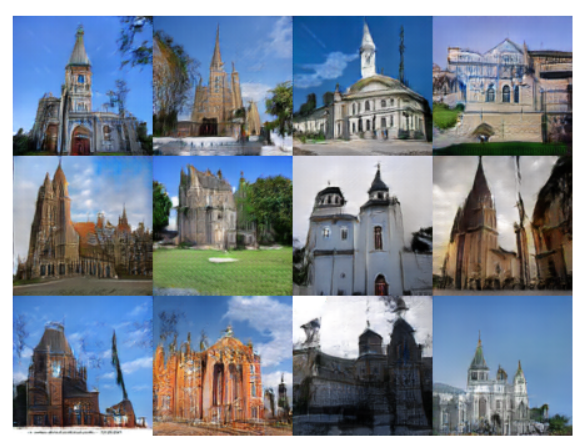
\includegraphics[width=0.8\linewidth]{LSGAN}
    \end{figure}
\end{frame}

\begin{frame}
  \frametitle{f-GAN}
  \begin{itemize}
    \item Let $\mathrm{Prob}(\mathcal{X})$ denote the space of probability
      measures defined on $\mathcal{X}$.
      For $\mathbb{P}, \mathbb{Q} \in \mathrm{Prob}(\mathcal{X})$
      assumed to be absolutely continuous,
      $f: \mathbb{R}_+\rightarrow\mathbb{R}$ a convex, lower-semicontinuous
      (i.e.\ its epigraph is closed) function satisfying $f(1) = 0$, we
      define the $f$-divergence,
      \[
        D_f(\mathbb{P}\|\mathbb{Q})
        = \int_{\mathcal{X}} Q(x)f\left(\frac{P(x)}{Q(x)}\right)dx.
      \]
    \item EX: Take $f: u\mapsto u\log u$ we get the KL divergence and take
      $f: u\mapsto (u-1)^2$ we get the reverse Pearson (if define as presented
      earlier).
  \end{itemize}
\end{frame}

\begin{frame}
  \frametitle{f-GAN}
  \begin{itemize}
    \item Let $\mathcal{T}$ be an arbitrary class of functions
      $T: \mathcal{X}\rightarrow\mathbb{R}$, we have:
      \[
        D_f(\mathbb{P}_r\|\mathbb{P}_{\theta})\ge
        \sup_{T\in\mathcal{T}}
        (\mathbb{E}_{x\sim\mathbb{P}_r}[T(x)]
        - \mathbb{E}_{x\sim\mathbb{P}_{\theta}}[f^{\thinspace *}(T(x))]),
      \]
      where $f^{\thinspace *}: s\mapsto\sup_{u\in\mathrm{dom}_f}(su-f(u))$
      is the Fenchel conjugate of $f$.
    \item We can therefore estimate a lower bound of
      $D_f(\mathbb{P}_r, \mathbb{P}_{\theta})$ by maximizing the above
      qunatity.
    \item Since $f^{\thinspace *}$ is not always defined over $\mathbb{R}$,
      we fix an `output activation function'
      $g_f: \mathbb{R}\rightarrow\mathrm{dom}_{f^{\thinspace *}}$ for each
      $f$ and define $T_w = g_f(V_w(x))$ where
      $V_w:\mathcal{X}\rightarrow\mathbb{R}$ is a function parameterized by
      $w$ without any range constraints on the output.
  \end{itemize}
\end{frame}

\begin{frame}
  \frametitle{Energy-based GAN}
  \begin{itemize}
    \item Output of $D$ is regarded as \textbf{energy}. $G$ is then trained
      to produce contrastive samples with minimal energies.
    \item Discriminator $D$ tries to minimize
      \[
        L_D(G, D) = \mathbb{E}_{x\sim\mathbb{P}_r}[D(x)]
        + \mathbb{E}_{z\sim\mathbb{P}_z}[[m - D(G(z))]^+]
      \]
      for some $m > 0$ and $[\cdot]^+=max(0, \cdot)$.
    \item Generator $G$ is trained to minimize
      \[ L_G(G, D) = \mathbb{E}_{z\sim\mathbb{P}_z}[D(G(z))]. \]
    \item $D$ is constrained to be non-negative.
  \end{itemize}
\end{frame}

\begin{frame}
  \frametitle{Energy-based GAN}
  \begin{itemize}
    \item Total variation (TV) distance between two probability measures
      $\mathbb{P}, \mathbb{Q} \in \mathrm{Prob}(\mathcal{X})$:
      \[
        \delta(\mathbb{P}, \mathbb{Q})
        = \sup_{A\in\Sigma} |\mathbb{P}(A)-\mathbb{Q}(A)|
        = \|\mathbb{P} - \mathbb{Q}\|_{TV},
      \]
      where $\Sigma$ is the set of all the Borel subsets of $\mathcal{X}$
      and $\|\cdot\|_{TV}$ denotes the total variation of a signed measure.
    \item We can show that training a EBGAN is equivalent to minimizing
      $\delta(\mathbb{P}_r, \mathbb{P}_{\theta})$.
    \item JS and TV induced the same topology on $\mathrm{Prob}(\mathcal{X})$
      (i.e.\ $\delta(\mathbb{P}_n, \mathbb{P})\rightarrow 0 \Leftrightarrow
        JS(\mathbb{P}_n, \mathbb{P})\rightarrow 0$).
    \item \textbf{EBGAN is not better than classical GAN.}
  \end{itemize}
\end{frame}

\section{Conclusion}

\begin{frame}
  \frametitle{Conclusion}
  \begin{itemize}
    \item Generaor + Descriminator/Critic/Energy function + Loss.
    \item WGAN: Well-done theoretical analysis and consistency
      between theory and practice.
    \item Many other extensions: InfoGAN, Conditional GAN, AdaGan,
      LAPGAN, BGAN, \ldots
    \item Applications: Super-resolution, Image inpainting, Style transfer,
      Semi-supervised learning, \ldots
  \end{itemize}
\end{frame}

\begin{frame}
  \frametitle{And You Can Train Your Own Models!}
  \begin{itemize}
    \item DCGAN (TensorFlow):
      \url{https://github.com/carpedm20/DCGAN-tensorflow}
    \item WGAN (PyTorch):
      \url{https://github.com/martinarjovsky/WassersteinGAN}
    \item ImprovedWGAN (TensorFlow):
      \url{https://github.com/igul222/improved_wgan_training}
    \item LSGAN (TensorFlow):
      \url{https://github.com/xudonmao/LSGAN}
    \item InfoGAN (TensorFlow):
      \url{https://github.com/openai/InfoGAN}
    \item And more \ldots
  \end{itemize}
\end{frame}

\renewcommand*{\bibfont}{\scriptsize}
\begin{frame}
  \frametitle{References}
  \nocite{*}
  \printbibliography
\end{frame}

\begin{frame}
  \vspace{1em}
  \begin{center}
    \Huge \color{BlueViolet}
    Thanks for your attention.
  \end{center}
\end{frame}
